\chapterimage{Chapter17.jpg} % Chapter heading image

\chapter{Wastewater Chemicals}

\section{Wastewater treatment chemicals - by use/category}\index{Wastewater treatment chemicals - by use/category}

\setlength{\arrayrulewidth}{0.1mm}
\setlength{\tabcolsep}{8 pt}
\renewcommand{\arraystretch}{1.3}
%{\rowcolors{2}{green!60!yellow!50}{green!30!yellow!40}
\begin{tabular}{ |p{5.5cm}|p{4.5cm}|p{5cm}|  }
\hline
% \multicolumn{3}{|c|}{\textbf{WASTEWATER TREATMENT CHEMICALS - BY USE/CATEGORY}} \\
% \hline
%\thead{A Head} & \thead{A Second \\ Head} & \thead{A Third \\ Head} \\
%\hline%

\hspace{0.5cm}USE/CATEGORY & \hspace{1.2 cm} PROCESS & \hspace{1.2 cm} CHEMICALS USED \\
\hline
pH Control/ \newline Alkalinity Supplement & Odor Control \newline Secondary Treatment \newline Digestion & Caustic soda \newline Magnesium hydroxide \newline Calcium oxide \newline Ammonia \newline Sodium carbonate \newline Muriatic acid\\
\hline
Oxidant & Odor Control \newline Disinfection & Chlorine \newline Sodium hypochlorite (NaOCl) \newline Calcium hypochlorite (HTH) \newline Hydrogen Peroxide\\
\hline
Advance Primary Treatment/ \newline Chemically Enhanced Primary Treatment (CEPT)/Phys-Chem & Primary Treatment & Ferric Chloride \newline Anionic Polymer\\
\hline
Filament Control & Secondary  & Bleach \newline Cationic Polymer\\
\hline
Phosphorous Removal  & Primary Treatment \newline Secondary Treatment & Iron Salts \newline Alum (Precipitant)\\
\hline
Nitrogen Removal  & Breakpoint Chlorination & Chlrorine \newline Sodium Hypochlorite\\
Dechlorination  & Disinfection & Sodium bisulfite  \newline Sulfur dioxide   \\
\hline
Flocculation/Solids Separation & Sludge Dewatering \newline Sludge Thickening & Cationic Polymer \\
\hline
Descaling & Odor Control Scrubber & Muriatic Acid \\
\hline
\end{tabular}

\newpage
\section{Wastewater treatment chemicals - by use/category}\index{Wastewater treatment chemicals - by use/category}
%{\rowcolors{2}{green!60!yellow!50}{green!30!yellow!40}
\begin{tabular}{ |p{4cm}|p{4.5cm}|p{6.5cm}|  }
\hline
% \multicolumn{3}{|c|}{\textbf{WASTEWATER TREATMENT CHEMICALS - BY PROCESS}} \\
% \hline
%\thead{A Head} & \thead{A Second \\ Head} & \thead{A Third \\ Head} \\
%\hline%

\hspace{1 cm}PROCESS & \hspace{1.2 cm} ACTION & \hspace{1.2 cm} CHEMICAL USED (ROLE) \\
\hline
Collections & Odor Control & Caustic Soda (pH control) \newline Magnesium Hydroxide (pH control) \newline Hydrogen Peroxide (Oxidant) \newline Sodium Nitrate (Biological Degradation)\newline Iron Salts (Precipitant)\\
\hline
Primary & CEPT & Ferric Chloride (Coagulant) \newline Anionic Polymer (Flocculant) \\
\hline
Secondary    &Filament Control \newline \textsf{} \newline WAS Thickening & Bleach \newline Cationic Polymer \newline Cationic Polymer (Flocculant)\\
\hline
Nutrient Removal & Phosphorous Removal \newline \textsl{} \newline
Alkalinity Supplementation & Iron Salts (Precipitant) \newline Alum (Precipitant)\newline Calcium Oxide \newline Ammonia \newline Sodium Carbonate \\
\hline
Tertiary Treatment & Disinfection  \newline 
Dechlorination & Chlorine/Bleach \newline Sodium Bisulfite  \newline Sulfur Dioxide   \\
\hline
Dewatering & Flocculation & Cationic Polymer \\
\hline
Plant Odor Control & Foul Air Scrubbing & Hydrogen Peroxide (Oxidant) \newline Bleach (Oxidant) \newline Caustic Soda (pH Control) \newline Muriatic Acid (pH Control \& Scrubber Descaling)\\
\hline
Anaerobic Digestion & Hydrogen Sulfide Control \newline Alkalinity Supplementation & Iron Salts (Precipitant) \newline Calcium Oxide \newline Ammonia \newline Sodium Carbonate \\
\hline
\end{tabular}

\section{Advance primary treatment (APT)}\index{Advance primary treatment (APT)}
Synonyms:  Advance primary treatment (APT), Chemically enhanced primary treatment (CEPT), Physical-chemical treatment (Phys-chem)
\subsection{Background}\index{Background}     
      
        \begin{itemize}
			\item Suspended solids present in wastewater are typically coated with bacterial slime and biological metabolic products which are negatively charged.  A significant portion of the suspended solids in wastewater do not settle easily due to gravity as:
				\begin{enumerate}
					\item the biological mass and the associated byproduct gases produced makes these particles buoyant, 
					\item the negative electrostatic charges on these particles cause these particles to be in constant state of motion due to electrostatic repulsion
				\end{enumerate}
			\item involves chemical addition to the primary influent flow to enhance primary treatment TSS and BOD removal efficiencies
			\item a normal primary treatment process typically removes 40 to 60\% TSS and 25 to 40\% BOD.  TSS and BOD removal efficiencies of over 80\% and 60\% respectively, may be achieved by the use of APT.
			\item additional cost incurred for the chemical addition is in most cases is offsetted by the benefits which include:
				\begin{enumerate}
					\item by removing more BOD in the primary treatment cost associated with secondary treatment is reduced
					\item primary BOD is more easy to digest than the secondary biomass thus the digester gas production is increased and digested solids production is lowered thus saving biosolids hauling cost
					\item residual ferric chloride in the primary sludge provides H$_2$S and struvite control in the solids treatment processes  
				\end{enumerate}
		\end{itemize}
\vspace{0.4 cm}

\subsection{Process/mechanism}\index{Process/mechanism}    

APT is a two step chemical process:

\subsection{Coagulation}\index{Coagulation}  
				                \begin{itemize}
									\item Coagulation is the process by which the negative charge on these particles is reduced lowering the repulsion forces, by the use of a chemical such as ferric chloride and alum.\\
									\item The concentration of the coagulant required is dependent on the strength of the wastewater and the conveyance time of the wastewater.
									\item Typically the coagulant is added immediately after the grit chambers so the conveyance from the grit chambers to the primary clarifier provides adequate contact time and mixing.\\
									\item Parameters to ensure optimal coagulation are:
										\begin{itemize}
											\item Appropriate coagulation concentration
											\item Adequate mixing energy, and
											\item Adequate contact time
										\end{itemize}
									\item Overdosing the coagulant will adversely effect the settleability.
									\item Typical ferric chloride dosage for coagulation range from 12 to 22 mg/l.
								\end{itemize}
\subsection{Flocculation}\index{Flocculation}  
			                	\begin{itemize}
									\item Flocculation uses an anionic polymer - polymer which has negatively charged groups, to bridge the coagulated particles to a size which will settle in the primary clarifier.  
									\item The flocculated particles are prone to shearing thus the polymer is gently folded in with the coagulated wastewater just prior to entry into the primary clarifier
								\end{itemize}
					

\vspace{0.6cm}
\hspace{6.8 cm} \textbf{CEPT Schematic}\\
\vspace{0.6cm}
\hspace{1.5 cm}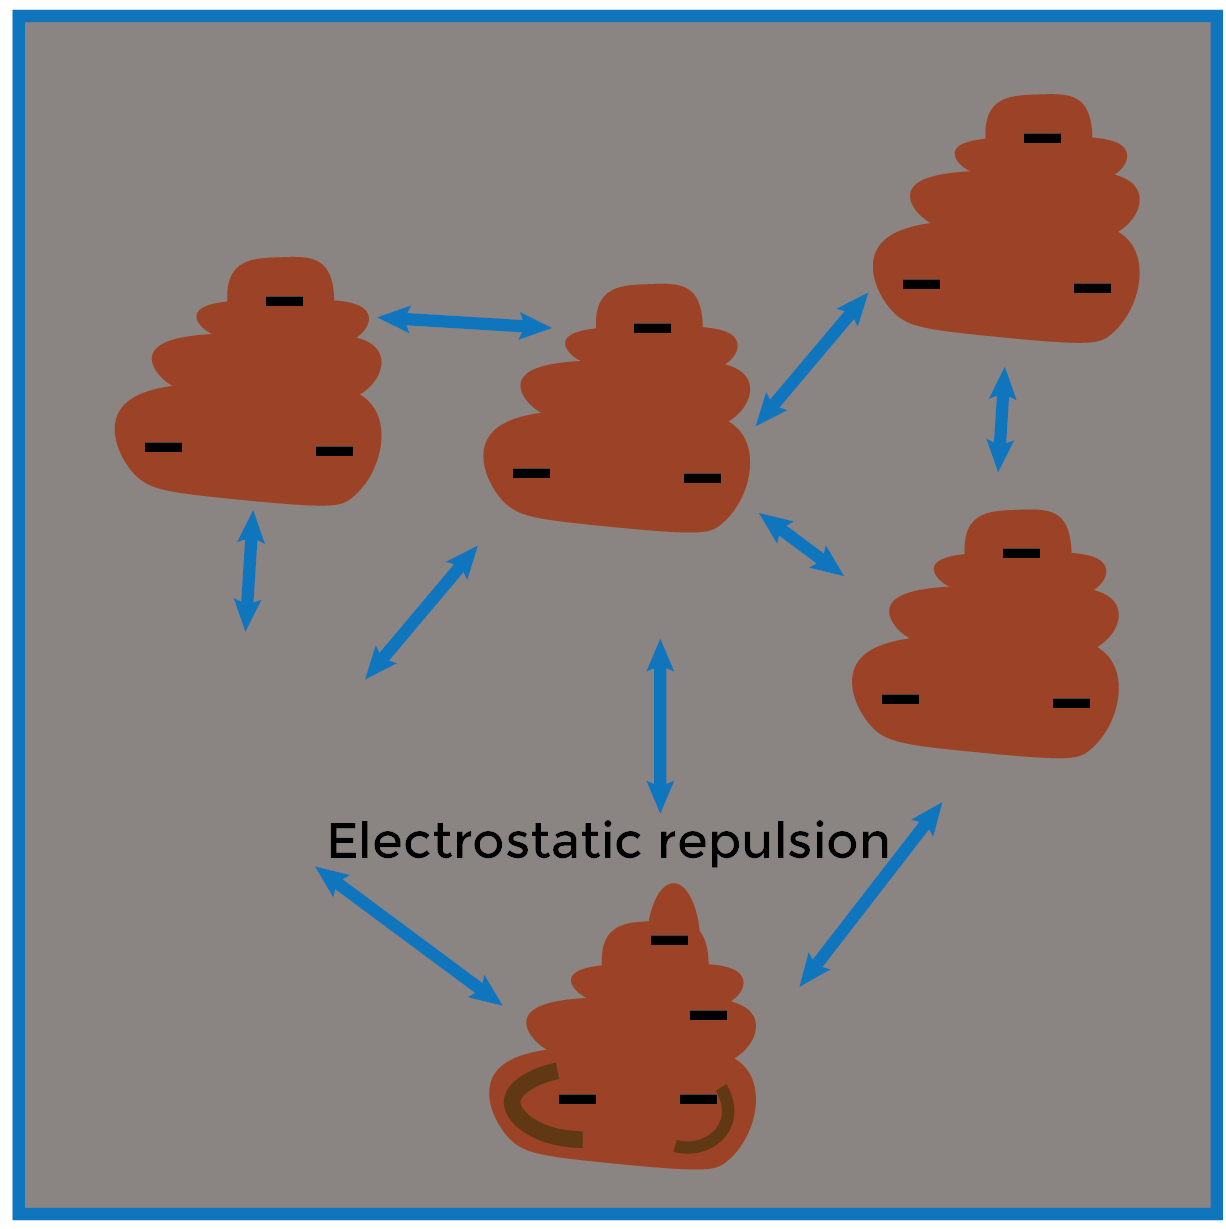
\includegraphics[scale=.13]{CEPTInitial} \hspace{0.7 cm}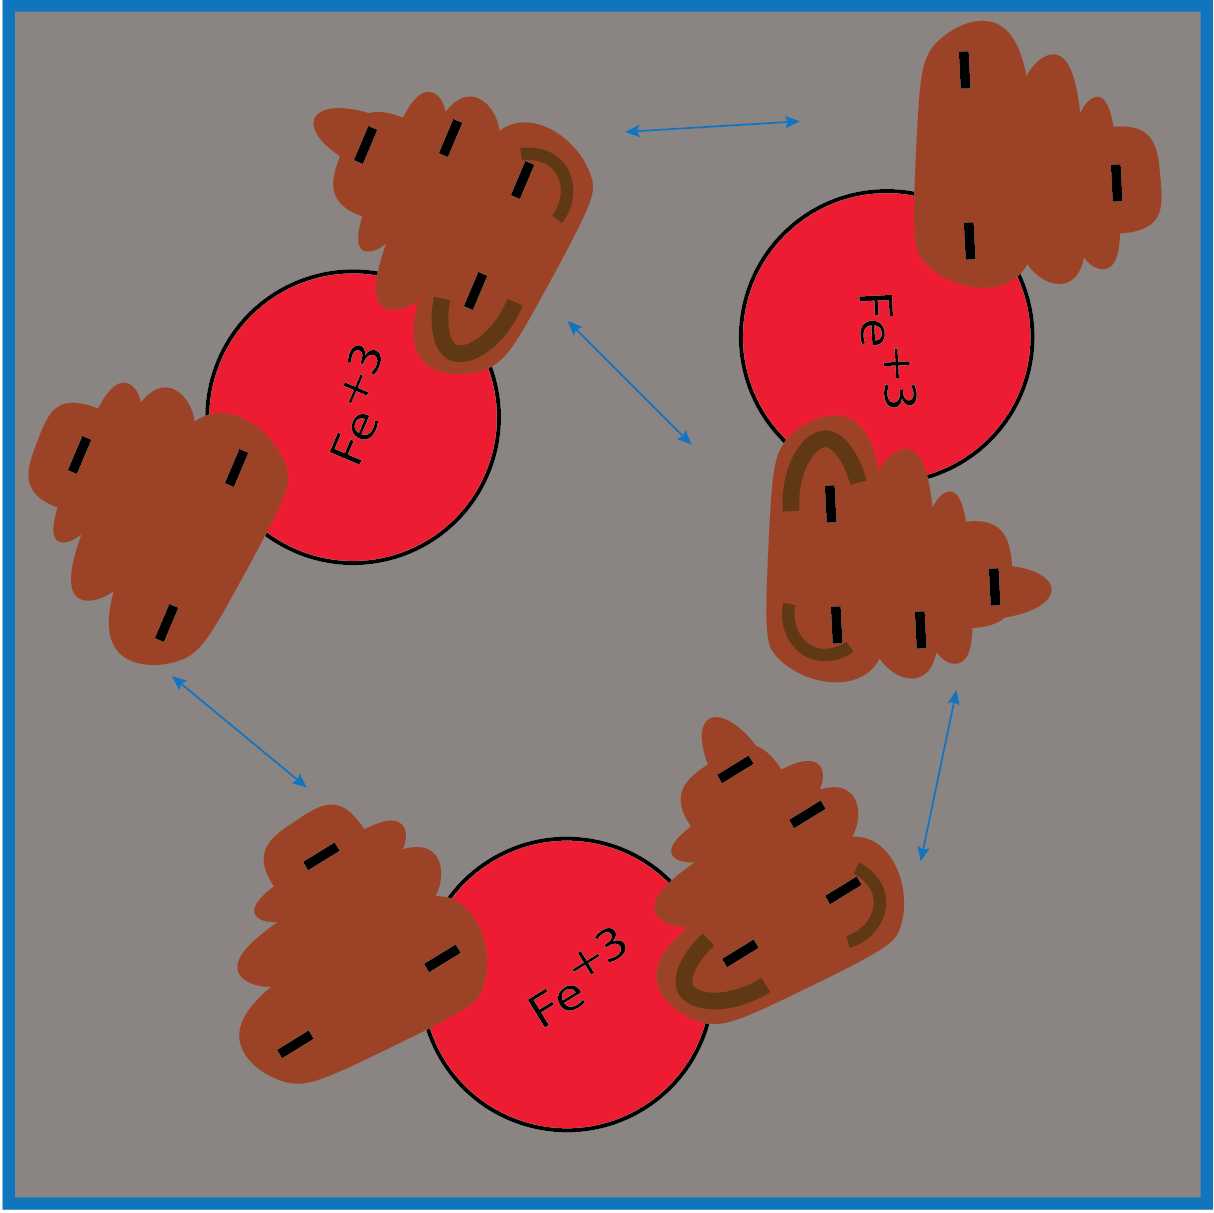
\includegraphics[scale=.13]{CEPTCoagulation}\hspace{0.7 cm}
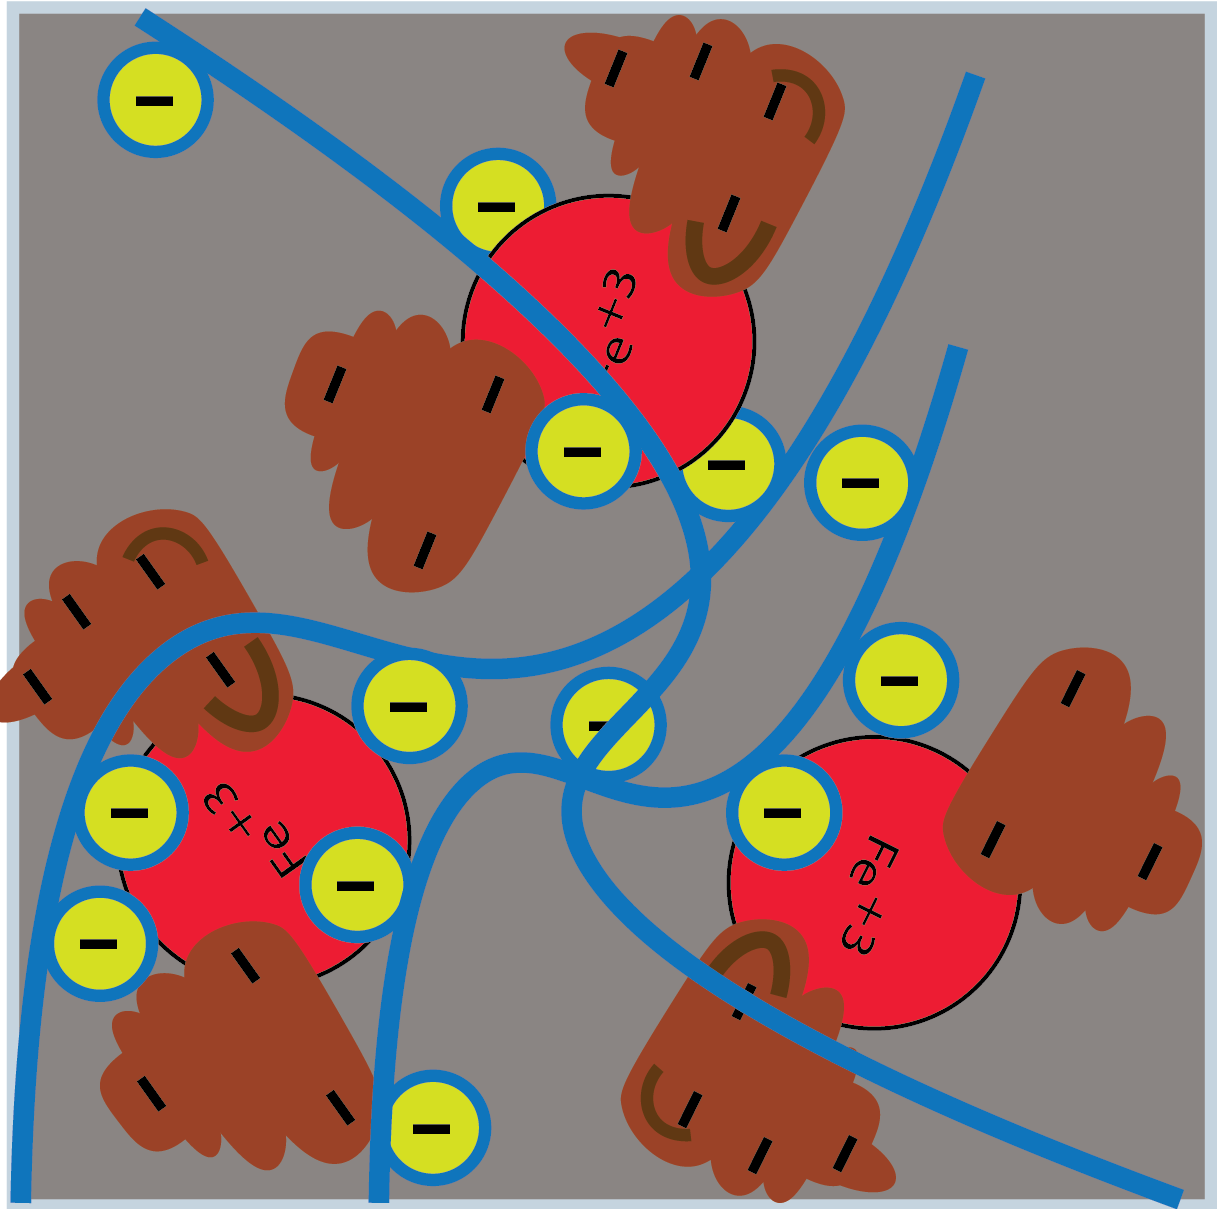
\includegraphics[scale=.13]{CEPTFlocculation}\\
\hspace{0.8 cm} \textbf{Untreated Primary Inluent}\hspace{1.6 cm}\textbf{Coagulation}\hspace{2.8 cm}\textbf{Flocculation}\\

\subsection{Polymers in wastewater treatment}\index{Polymers in wastewater treatment} 
        	\begin{itemize}
        		\item Polymer use in wastewater treatment includes:
        			\begin{itemize}
        				\item For enhancing primary removal efficiencies
        				\item For sludge thickening - to increase the solids content of the sludge feed to the digester
        				\item For solids dewatering - to reduce the digested solids hauling cost and to make the final solids product more manageable
        				\item For filament control in activated sludge treatment
        			\end{itemize}
        	\end{itemize}
  

\vspace{0.6cm}
Both anionic and cationic polymers used in wastewater treatment are available in the following forms: 
\begin{enumerate}
\item Dry Polymers:  These are available in granular, flake or bead form and have an active polymer as high as 95\%.  Prior to use, the dry polymers have to be dissolved in water using specialized mixing units 
\item Emulsion Polymer:  This water soluble version consists of water droplets dispersed in oil.  They have 25\% to 50\% active polymer content and require a specialized system to disperse it in water prior to use.
\item Solution polymers:  These are water soluble polymers in water. These polymers are relatively easy to put into dilute solution.  However, the lower active polymer content increases the shipping cost of this type of polymer.
\item Cationic polymer is also available as a low cost solution type polymer - Mannich Polymer (mannich is a type of chemical reaction involving formalydehyde which is used for making this polymer).  However, it has certain drawbacks which include: 
\begin{enumerate}
\item Presence of formaldehyde which lends its offensive odor
\item Higher viscosity which imposes operational challenges related to its use, and
\item High pH which leads to formation of hardness deposits in the associated piping and equipment.
\end{enumerate}
\end{enumerate}

The polymers use is primarily a function of the process stream.  Each system is different and there are no hard and fast rules regarding which products will work and therefore jar tests and pilot tests are conducted as part of the product selection process.\\

\section{Chemical dosing math problems}\index{Chemical dosing math problems}
\subsection{lbs chemicals needed given flow and dosing rate}\index{lbs chemicals needed given flow and dosing rate}

\begin{itemize}
\item Use lbs formula to calculate the lbs of chemicals required\\
\item Using the calculated lbs chemical required value, calculate the amount of that chemical at the concentration available
\end{itemize}

So for example, if asked how much many gallons per day of bleach solution (SG 1.2)containing 12.5\% available chlorine is required to disinfect a 10 MGD flow of water given the required chlorine dosage of 7 mg/l.\\
\begin{enumerate}
\item calculate the lbs of chlorine required using the lbs formula:\\
\vspace{0.5cm}
=$10 MGD \enspace * \enspace 7 \dfrac{mg}{l} \enspace * \enspace 8.34\enspace=\enspace 583.8 \enspace lbs \enspace chlorine \enspace per \enspace day$\\
\vspace{0.5cm}
\item calculate the gallons of bleach which will provide the 583.3 lbs chlorine\\
\vspace{0.5cm}
Applying the lbs formula - note that 8.34 * SG will give the actual lbs/gal of bleach.  If SG is not provided, use only 8.34 lbs per gallon:\\
\vspace{0.5cm}
$583.3 \dfrac{lbs \enspace bleach}{day}\enspace=\enspace x \dfrac{gal}{day} \enspace * \enspace 8.34 * 1.2 \dfrac{lbs \enspace bleach}{gal} \enspace * \enspace 0.0125 \dfrac{lbs \enspace chlorine}{lb \enspace bleach} \enspace $\\
\vspace{0.5cm}
$ \implies x \dfrac{gal}{day}\enspace = \enspace \dfrac{583.3}{8.34*1.2*0.125} \enspace = \boxed{466 \dfrac{gal}{day}}$
\end{enumerate}

\subsection{Chemical batching and dilution}\index{Chemical batching and dilution}

These problems include questions such as:  \textit{How much initial volume of a 4\% polymer solution is needed to make 3500 gallons of polymer at 0.25\% concentration?}\\
\begin{itemize}
\item These type of problems are solved using C*V relationship where C is the concentration and V is the volume.

\item As C is expressed in weight/volume, C*V will equal to weight.  The weight of the chemical will be same before and after the dilution

\item If C$_1$ is the concentration of the chemical before dilution and V$_1$ is the volume of that initial concentration that is needed and C$_2$ is the final concentration that you want to make and V$_2$ is the volume that you are making of the final concentration, C$_1$ * V$_1$ = C$_2$ * V$_2$.

\item Knowing C$_1$, C$_2$ and V$_2$, we can calculate V$_1$ as: $$V_1 = \dfrac{C_2 * V_2}{C_1}$$

$$V_{4\%} = \dfrac{C_{.25\%} * V_{.25\%}}{C_{4\%}} = \dfrac{0.25 \enspace * \enspace 3500}{4}= 219 gal $$ 

Take 219 gallons of the 4\% polymer and dilute to 3,500 gallons to give a 0.25\% polymer solution.

\end{itemize}